\section{Auswertung}
\label{sec:Auswertung}

\subsection{Überprüfung der Stabilitätsbedingung}

\begin{figure}
  \centering
  \includegraphics{stability.pdf}
  \caption{Stabilitätsbedingung für die verwendeten Spiegelkonfigurationen.}
  \label{fig:stability}
\end{figure}

\begin{table}
  \centering
  \aboverulesep=0ex % Solution part 1 of 3
  \belowrulesep=0ex % Solution part 1 of 3
  \caption{Messdaten zur Überprüfung der Stabilitätsbedingung für beide Spiegelkonfigurationen.}
  \label{tab:stability}
  \begin{tabular}{S[table-format = 3.0] S[table-format = 1.1] | S[table-format = 3.1] S[table-format = 1.1]}
    %\toprule
    \multicolumn{2}{c}{$r_2 = \qty{1400}{\milli\metre}$} & \multicolumn{2}{c}{$r_2 = \infty$} \\
    \midrule
    \rule{0pt}{1.1EM}
    {$L \mathbin{/} \unit{\centi\metre}$} & {$I \mathbin{/} \unit{\milli\watt}$} & {$L \mathbin{/} \unit{\centi\metre}$} & {$I \mathbin{/} \unit{\milli\watt}$}\\
    \midrule
    \rule{0pt}{1.1EM}
     50 & 3.0 &    55 & 4.8 \\
     75 & 4.0 &    70 & 2.0 \\
    100 & 2.8 &    96 & 2.4 \\
    125 & 2.7 &   120 & 4.3 \\
    150 & 2.2 &   131 & 3.2 \\
    175 & 3.3 & 134.5 & 2.7 \\
    200 & 2.0 & 137.5 & 1.0 \\
        &     &   140 & 1.0 \\
        &     &   141 &   0 \\ 
    %\bottomrule
  \end{tabular}
\end{table}

\subsection{Messung der TEM Moden}

\begin{table}
  \centering
  \aboverulesep=0ex % Solution part 1 of 3
  \belowrulesep=0ex % Solution part 1 of 3
  \caption{Messdaten der Intensitätsverteilung der $\text{TEM}_{00}$ und $\text{TEM}_{01}$ Moden.}
  \label{tab:TEM}
  \begin{tabular}{S[table-format = 2.0] | S[table-format = 1.3]  S[table-format = 1.2]}
    %\toprule
    {} & {$\text{TEM}_{00}$} & {$\text{TEM}_{00}$} \\
    \midrule
    \rule{0pt}{1.1EM}
    {$d \mathbin{/} \unit{\milli\metre}$} & {$I \mathbin{/} \unit{\micro\ampere}$} & {$I \mathbin{/} \unit{\micro\ampere}$} \\
    \midrule
    \rule{0pt}{1.1EM}
    -20 & 0.015 & 0.03 \\
    -18 & 0.021 & 0.03 \\
    -16 & 0.025 & 0.01 \\
    -14 & 0.034 & 0.01 \\
    -12 & 0.062 & 0.04 \\
    -10 & 0.28  & 0.12 \\
     -9 & 0.43  & 0.20 \\
     -8 & 0.74  & 0.31 \\
     -7 & 1.11  & 0.42 \\
     -6 & 1.53  & 0.55 \\
     -5 & 2.08  & 0.69 \\
     -4 & 2.8   & 0.73 \\
     -3 & 3.3   & 0.70 \\
     -2 & 3.7   & 0.58 \\
     -1 & 3.6   & 0.40 \\
      0 & 3.6   & 0.25 \\
      1 & 2.9   & 0.10 \\
      2 & 2.4   & 0.02 \\
      3 & 1.5   & 0.05 \\
      4 & 0.96  & 0.17 \\
      5 & 0.36  & 0.31 \\
      6 & 0.20  & 0.42 \\
      7 & 0.14  & 0.53 \\
      8 & 0.10  & 0.54 \\
      9 & 0.068 & 0.56 \\
     10 & 0.047 & 0.50 \\
     12 & 0.018 & 0.35 \\
     14 & 0.009 & 0.17 \\
     16 & 0.006 & 0.09 \\
     18 & 0.005 & 0.03 \\
     20 & 0.004 & 0.02 \\
    %\bottomrule
  \end{tabular}
\end{table}

\subsubsection{$\text{TEM}_00$-Mode}

\begin{figure}
  \centering
  \includegraphics{TEM00.pdf}
  \caption{Messdaten der Intensitätsverteilung der $\text{TEM}_00$ Mode und Fit mittels \textit{scipy} \cite{scipy}.}
  \label{fig:TEM00}
\end{figure}

\subsubsection{$\text{TEM}_01$-Mode}

\begin{figure}
  \centering
  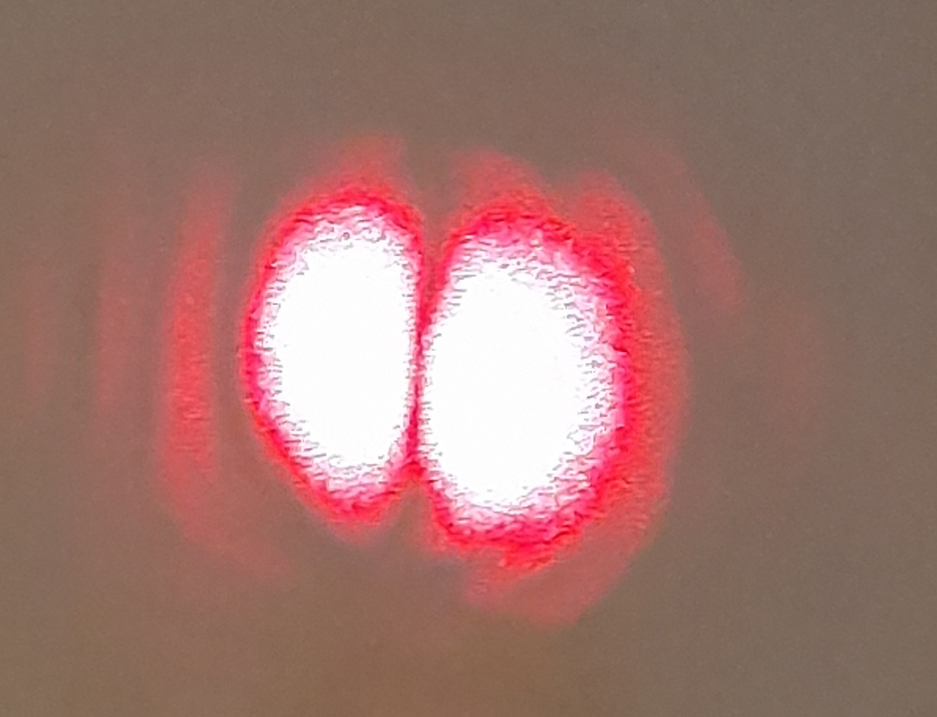
\includegraphics{TEM01.pdf}
  \caption{Messdaten der Intensitätsverteilung der $\text{TEM}_01$ Mode und Fit mittels \textit{scipy} \cite{scipy}.}
  \label{fig:TEM01}
\end{figure}

\subsection{Polarisation des Lasers}

\begin{table}
  \centering
  \aboverulesep=0ex % Solution part 1 of 3
  \belowrulesep=0ex % Solution part 1 of 3
  \caption{Messdaten zur Bestimmung der Polarisation des Laserstrahls}
  \label{tab:polarisation}
  \begin{tabular}{S[table-format = 3.0] S[table-format = 1.1] | S[table-format = 3.0] S[table-format = 1.1] | S[table-format = 3.0] S[table-format = 1.1]}
    %\toprule
    {$\theta \mathbin{/} \unit{\degree}$} & {$I \mathbin{/} \unit{\milli\watt}$} & {$\theta \mathbin{/} \unit{\degree}$} & {$I \mathbin{/} \unit{\milli\watt}$} &%
    {$\theta \mathbin{/} \unit{\degree}$} & {$I \mathbin{/} \unit{\milli\watt}$} \\
    \midrule
    \rule{0pt}{1.1EM}
      0 & 0.5 & 130 & 0.8 & 250 & 3.2 \\
     10 & 0.9 & 140 & 0.4 & 260 & 3.0 \\
     20 & 1.4 & 150 & 0.1 & 270 & 2.8 \\
     30 & 2.0 & 160 & 0.1 & 280 & 2.3 \\
     40 & 2.4 & 170 & 0.2 & 290 & 1.8 \\
     50 & 2.8 & 180 & 0.4 & 300 & 1.3 \\
     60 & 3.0 & 190 & 0.9 & 310 & 0.8 \\
     70 & 3.2 & 200 & 1.4 & 320 & 0.4 \\
     80 & 3.1 & 210 & 1.9 & 330 & 0.1 \\
     90 & 2.7 & 220 & 2.5 & 340 & 0.1 \\
    100 & 2.3 & 230 & 2.9 & 350 & 0.2 \\
    110 & 1.8 & 240 & 3.1 & 360 & 0.5 \\
    120 & 1.3 &     &     &     &     \\
    %\bottomrule
  \end{tabular}
\end{table}

\begin{figure}
  \centering
  \includegraphics{polarisation.pdf}
  \caption{Messdaten zur Bestimmung der Polarisation des Laserstrahls und Fit mittels \textit{scipy} \cite{scipy}.}
  \label{fig:polarisation}
\end{figure}

\subsection{Multimoden Betrieb}

\begin{table}
  \centering
  \aboverulesep=0ex % Solution part 1 of 3
  \belowrulesep=0ex % Solution part 1 of 3
  \caption{Frequenzspektrum $[f]$ des Lasers bei verschiedenen Resonatorlängen $L$.}
  \label{tab:Multimoden}
  \begin{tabular}{c | c | l}
    %\toprule
    {$L \mathbin{/} \unit{\centi\metre}$} & $[f] \mathbin{/} \unit{\mega\hertz}$ & $\symup{\Delta}f \mathbin{/} \unit{\mega\hertz}$ \\%& {$L_\text{exp} \mathbin{/} \unit{\centi\metre}$}\\
    \midrule
    \rule{0pt}{1.1EM}
     50 &                      {304, 611, 919} & {307,50 \pm \; 0,50} \\   
     \midrule
     \rule{0pt}{1.1EM} 
     75 &           {203, 405, 604, 806, 1009} & {201,50 \pm \; 1,50} \\    
     \midrule
     \rule{0pt}{1.1EM} 
    100 & {150, 300, 454, 600, 754, 904, 1054} & {150,67 \pm \; 2,75} \\   
    \midrule
    \rule{0pt}{1.1EM}  
    125 & {124, 240, 364, 480, 600, 720, 840,} & {120,00 \pm \; 2,67} \\  
        &                    {960, 1080, 1204} &                      \\   
    \midrule
    \rule{0pt}{1.1EM}  
    150 & {101, 203, 304, 401, 503, 604, 701,} & {100,64 \pm \; 1,77} \\     
        &         {803, 904, 1005, 1106, 1208} &                      \\
    \midrule
    \rule{0pt}{1.1EM}
    175 &  {86, 176, 260, 350, 435, 518, 600,} & { 86,25 \pm \; 3,03} \\   
        &     {686, 773, 863, 949, 1031, 1121} &                      \\
    \midrule
    \rule{0pt}{1.1EM}
    200 &  {75, 154, 221, 300, 375, 450, 525,} & { 75,31 \pm \; 4,18} \\
        & {596, 670, 754, 825, 904, 980, 1054} &                      \\
  \end{tabular}
\end{table}

\subsection{Bestimmung der Wellenlänge des Lasers}

\begin{table}
  \centering
  \aboverulesep=0ex % Solution part 1 of 3
  \belowrulesep=0ex % Solution part 1 of 3
  \caption{Messdaten zur Bestimmung der Wellenlänge und resultierende Wellenlängen. Zu jeder Gitterkonstanten $g$ ist der Abstand der Maxima $n$-ter Ordnung 
  und die daraus resultierende Wellenlänge angegeben.}
  \label{tab:wellenlänge}
  \begin{tabular}{S[table-format = 4.0] | S[table-format = 3.0] | S[table-format = 1.0] | S[table-format = 2.1] | S[table-format = 3.2]}
    %\toprule
    {$g \mathbin{/} \unit{\milli\metre^{-1}}$} & {$d \mathbin{/} \unit{\centi\metre}$} & {$n$} & {$d_{nn} \mathbin{/} \unit{\centi\metre}$} & {$\lambda \mathbin{/} \unit{\nano\metre}$} \\
    \midrule
    \rule{0pt}{1.1EM}
    1200 & 25  & 1 &   58 & 631.18 \\
    \midrule
    \rule{0pt}{1.1EM}
     600 & 25  & 1 & 20.5 & 632.26 \\
         &     & 2 & 59.5 & 637.98 \\
    \midrule
    \rule{0pt}{1.1EM}
     100 & 80  & 1 &   10 & 623.78 \\
         &     & 2 & 20.5 & 635.43 \\
         &     & 3 &   31 & 634.04 \\
         &     & 4 &   42 & 634.75 \\
    \midrule
    \rule{0pt}{1.1EM}
      60 & 110 & 1 & 11.5 & 652.52 \\
         &     & 2 & 22.5 & 635.89 \\
         &     & 3 & 33.5 & 627.24 \\
    %\bottomrule
  \end{tabular}
\end{table}

